\documentclass{msuposter}
\usepackage{lipsum}
\usepackage{tikz,wrapfig}
\usepackage{algorithm}
\usepackage{algorithmic}
%% REQUIRED
\title{Using GANs to Generate Synthetic Data}
\author{Joseph Despres and Yunus Shariff}
\institute{Michigan State University}


%% SET COLUMN WIDTH
\newcommand{\colwidth}{0.3\linewidth}

\begin{document}
\begin{frame}{}
\begin{columns}[t]

\begin{column}{\colwidth}

\begin{block}{Introduction and Motivation}
The aim of this project is to extend the Generative Adversarial Network beyond image generation into generating synthetic data. The objective of any GAN is to train a Neural Network to recognize a fake, while training an adjacent Neural Network to spot the fake, the model has converged to a desirable solution where fake data are indistinguishable from the real \cite{NIPS2014_5ca3e9b1}.  This area has shown substantial progress in the past several years today's GANs are known to generate astonishingly accurate generating images. Applications for this technology have yet to be fully realized. This project explores one of many potential use cases.

\end{block}

\begin{block}{Potential Use Cases}

Although data are more and more available in seeming abundance, there is still a need to generate more. First, big datasets are often convenient to collect and not controlled.

\begin{itemize}
	\item \textbf{Use to generate additional datapoints in Controlled experiments}
\end{itemize}

Since These data will be generated, confidentially is less of a concern. Therefore, these data could be used by peole training models outside of a pariticular organization.

\begin{itemize}
	\item \textbf{Use to generate data to fit models where data are confidential}
	
\end{itemize}

\end{block}

\begin{block}{Method}

The challenges with training a GAN to generate synthetic data is a row in a dataframe is several orders of magnitude smaller than a full image. An artificial nerual network has no difficulty fitting to it. The challenge is getting the right fit. This is a ballance between fitting the data so well it mimics the data seen and underfitting where it cannot generate. Therefor  where the process could be generative yet, 

\begin{figure}
  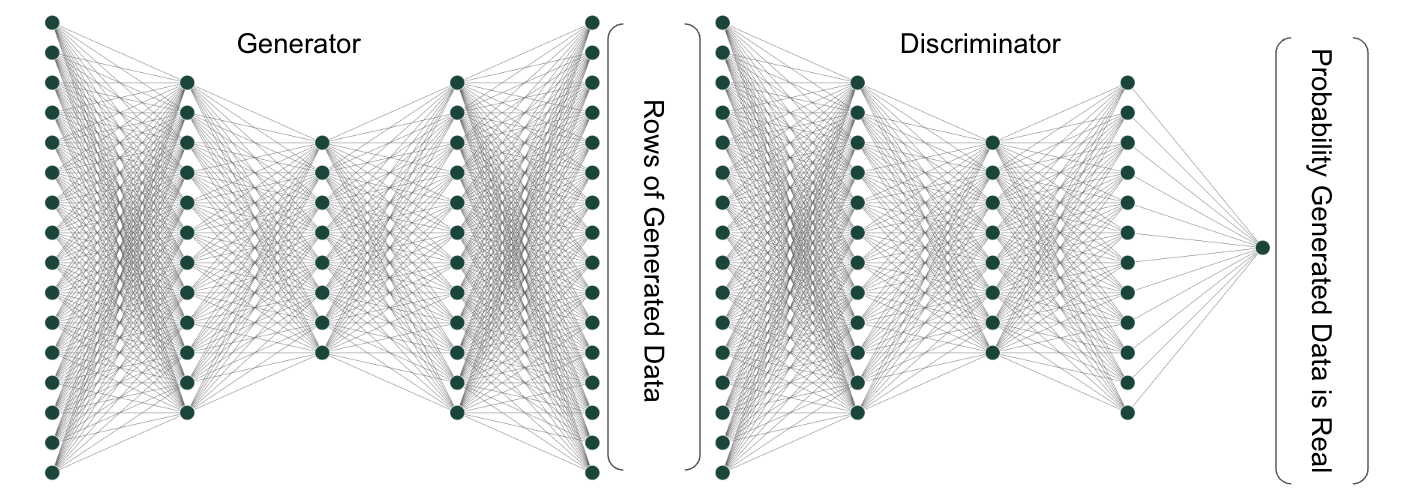
\includegraphics[width=\linewidth]{gan_diag.png}
\end{figure}

\newpage 



\end{block}. 


\end{column}

%% COLUMN DIVIDE %%%%%%%%%%%%%%%%%%%%%%%%%%%%

\begin{column}{\colwidth}

\begin{block}{Experiment}

\begin{figure}
  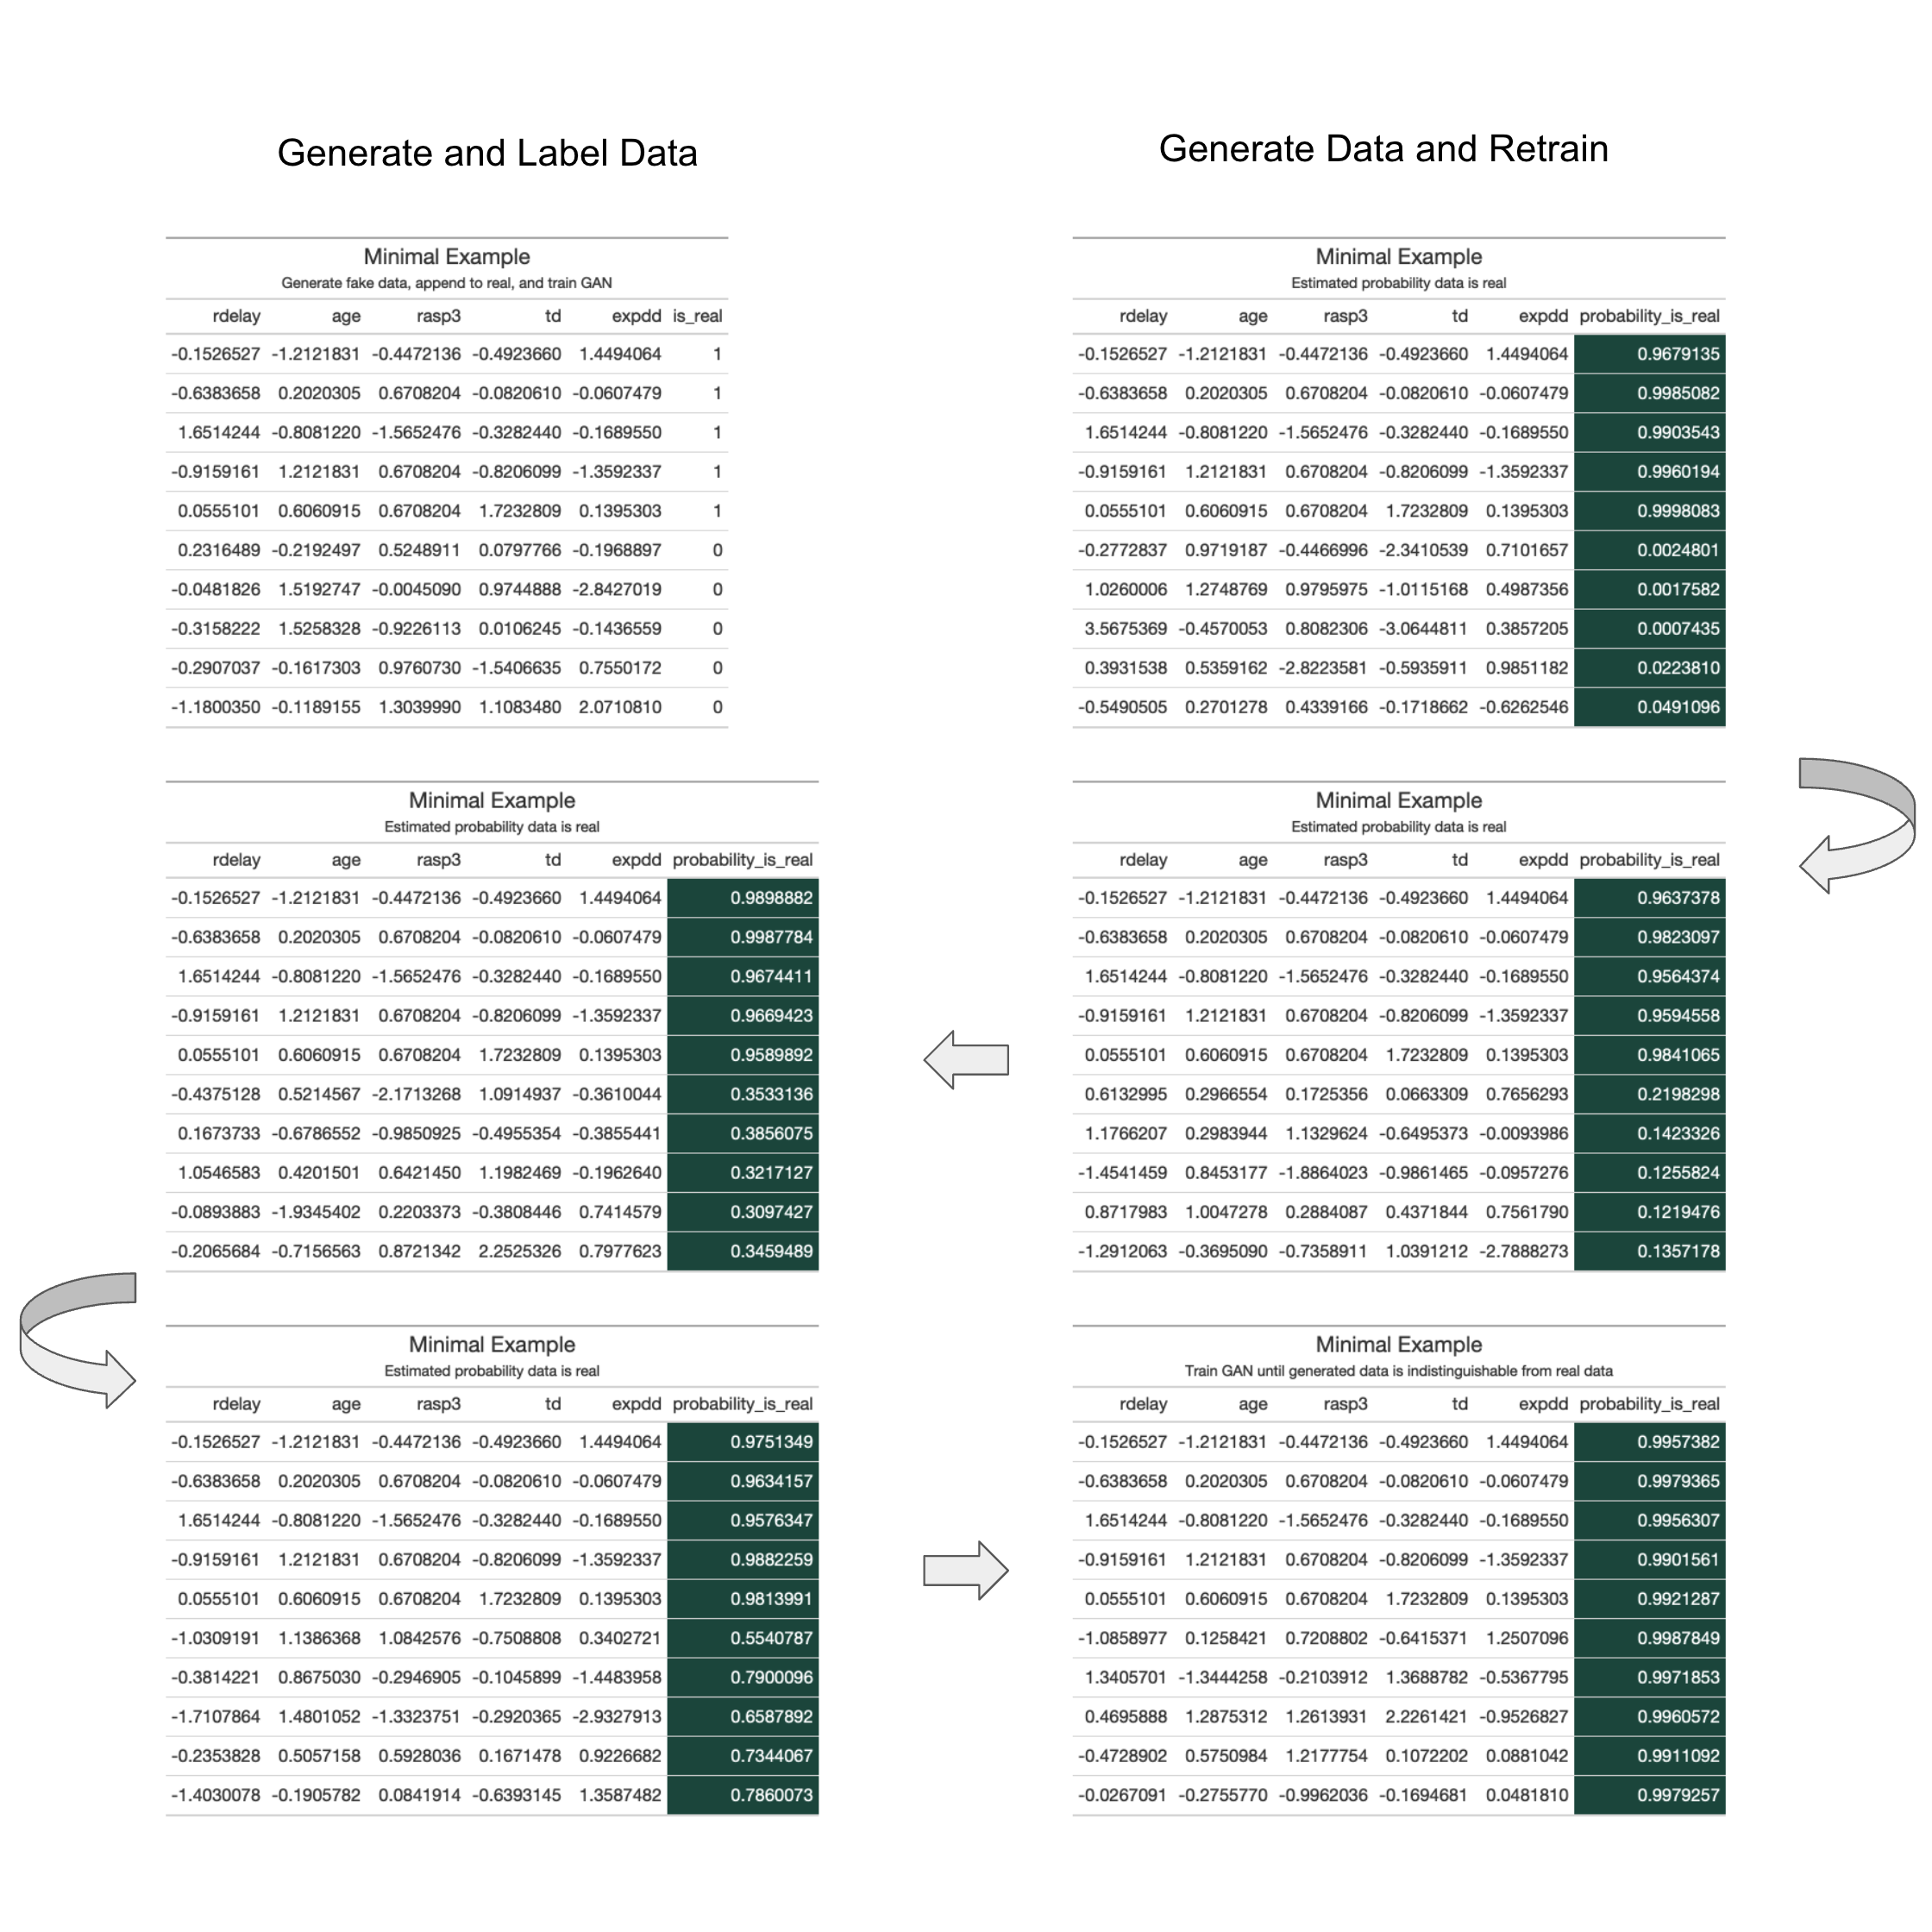
\includegraphics[width=\linewidth]{gan_conv.png}
\end{figure}

This project we use New York City Taxi from 2016. Primarily because of well collected. data from the N 

\cite{nyc2016}

\end{block}

\begin{block}{Results}

\end{block}


\end{column}

%% COLUMN DIVIDE %%%%%%%%%%%%%%%%%%%%%%%%%%%%

\begin{column}{\colwidth}


\begin{block}{References}
\scriptsize
\bibliography{references}
\bibliographystyle{plain}
% \end{scriptsize}
\end{block}

%%%% end of references %%%%%%%%%%%%%%%%
\end{column}

\end{columns}
	\end{frame}
\end{document}
